\chapter{Literature review}


\section{Segmentation and image objects}
On the Earth's surface, we have both man-made and natural objects such as trees, houses, rivers, roads, mountains, and forests, among others. These geographic objects are typically represented on satellite images by pixels, which, in reality, provide an unnatural representation because most features are irregular in shape and size. Additionally, at lower resolutions, a single pixel often represents a mix of features, while high-resolution images exhibit high intra-class variability.

In Object-Based Image Analysis (OBIA), images are divided into regions or segments, known as image objects, through a process called segmentation. The goal is to obtain regions that closely align with features on the Earth's surface by grouping pixels based on homogeneity criteria. The measure of alignment is assessed by the homogeneity of segments, boundary adherence, and the impact segments have on subsequent image processes\cite{audebert_how_2016}.

Objects offer several advantages over pixels. Firstly, objects provide a meaningful representation of ground features. Secondly, unlike pixels, which rely solely on spectral characteristics for feature mapping, objects allow for the incorporation of contextual information such as shape, texture, geometry, and neighborhood topologies\cite{lang_object_2010}. Furthermore, objects enable the incorporation of ancillary data into image analysis\cite{kressler_object-oriented_2008}.

Despite the significant potential of utilizing objects in deep learning, especially for high-resolution images, it remains relatively uncommon due to the technical expertise required. High-resolution images pose practical challenges for deep networks, mainly due to the substantial computational resources they demand. Consequently, preprocessing these images is a necessary step to make them manageable for deep learning models. Two prevalent preprocessing methods are extracting image patches using sliding windows and segmentation. Sliding windows involve systematically cropping smaller patches from the larger image, which can then be fed into the network. However, this approach might miss contextual information across the image boundaries. On the other hand, segmentation divides the image into meaningful regions or objects, which is particularly useful in object-based image analysis\cite{hao_land-use_2024}. 

Today, several algorithms are utilized for generating segments or regions from images, each employing distinct methods that categorize them into edge-based, region-based and hybrid methods. Edge-based techniques typically identify edges in an image and close them using contouring algorithms. On the other hand, region-based methods either start from an initial object and expand outward until a boundary is met (region merging), or begin with the entire image and split it based on the homogeneity of regions until only homogeneous regions remain (region splitting). Hybrid methods combine elements of both edge-based and region-based approaches to leverage their respective strengths and overcome their limitations \cite{hossain_segmentation_2019}.

Superpixel generation algorithms are a specialized category within these methods, focusing on dividing the image into smaller, homogeneous regions that align well with object boundaries. These algorithms also allow control over the number of superpixels generated\cite{stutz_superpixels_2018}. The most used superpixel generation algorithms include Simple Linear Iterative Clustering (SLIC), Quickshift, Felzenszwalb and Huttenlocher(FH) algorithm among others.

\subsection{SLIC}
This clustering-based technique utilizes k-means clustering to generate superpixels. Initially, it places a seed pixel on a regular grid, spaced $S$ pixels apart, creating a grid-like structure for the superpixels. At the start, there are $K$ cluster centers, each defined by spatial proximity, color information in the CIELAB or RGB color space. For multispectral images, SLIC can be extended to incorporate additional spectral bands thus utilizing the full range of spectral data available. The algorithm then proceeds by clustering the pixels within a $3 \times 3$ neighborhood, gradually expanding a region based on spatial and spectral homogeneity criteria. To manage computational complexity, the neighborhood search is confined to a $2S \times 2S$ area. The resulting superpixels are compact, nearly uniform, and respect image boundaries \cite{achanta_slic_2012}.


\subsection{Quickshift}
Similar to SLIC, Quickshift is also clustering-based, but it utilizes kernels to find clusters in the color and spatial spaces. Within this technique, the Parzen density estimate \( P_{x} \) is first computed, and then the algorithm moves each point towards the nearest neighbor for which there is an increment in density. Eventually, all points are connected into a single tree, and modes are recovered by breaking branches longer than a threshold.\cite{vedaldi_quick_2008}

\subsection{Felzenszwalb and Huttenlocher algorithm}
This edge-based segmentation algorithm operates by recursively merging neighboring image regions that have similar properties, such as color and texture. It utilizes a graph to represent the image, where each node corresponds to a pixel, and the edges connect pairs of neighboring pixels. The weights associated with these edges represent dissimilarities between pixels, such as spectral intensities and location.

The algorithm acknowledges that high variability in an image does not necessarily guarantee multiple regions, meaning regions may not always have nearly constant or slowly varying intensities. Therefore, breaking edges with large weights may not be appropriate. It is essential to consider spectral differences between boundaries and the global variations between neighboring regions.

The criterion for segmentation is adaptively adjusted based on the degree of variation between neighboring regions. This ensures that low-variability images preserve details while high-variability images can discard insignificant details.

Segmentation partitions the set of vertices into components, where each component corresponds to a connected component in the graph. Elements in the same component should be similar, meaning that edges between two vertices in the same component should have relatively low weights, and vice versa for different components\cite{felzenszwalb_efficient_2004}

\section{Feature extraction}
Once an image has been segmented, the question arises as to what these objects are. Semantic segmentation addresses this by assigning classes to the segments, thereby providing semantic meaning to the objects. To accomplish this, it is crucial to understand the patterns and characteristics associated with each class that will allow a model to distinguish these classes. These patterns, descriptors or characteristics of the raw data are known as object features.

Feature extraction is aimed at finding a feature vector that encapsulates the essential aspects of the input data. The feature vector is vital for recognizing image objects. It can be constructed by computing numerical features based on some expert knowledge. These are handcrafted features. With deep features, a neural network automatically learns from the data and extract its characteristics. These do not require any expert knowledge. While most studies have focused on extracting features from regular image patches, only a few have concentrated on objects themselves. Object-based approaches leverage object shapes to extract spatial information, which often leads to improved classification accuracy.


\subsection{Handcrafted feature extraction}
Handcrafted features are some of the most robust and interpretable features. The idea is to describe the spectral, textural, geometric and spatial characteristics of an image. Colour is one of the most important features in many image analysis tasks owing to its discriminative power and semantic relevance. It often exhibits relatively invariant characteristics with respect to changes in image size and object orientation. For instance, the color of a homogeneous object remains consistent regardless of its position within an image or its orientation. 

Descriptors that encapsulate the color distribution in an image, such as color moments, play a crucial role in image analysis. Color moments, including the first-order mean, second-order variance, and third-order skewness, are computed for each color band or as an average across all bands. Similarly, fuzzy moments, which incorporate spatial distribution, offer insights not only into the color distribution but also into the texture of an image. Additionally, color histograms describe the frequency of pixel values in an object, providing further detail about the color distribution\cite{tiwari_feature_2013}.

To describe the smoothness or roughness of an object based on its spectral distribution, various textural descriptors are employed. These descriptors include Gabor Filters \cite{grigorescu_comparison_2002}, Haar Wavelets \cite{raju_texture_2008}, Haralick features \cite{porebski_haralick_2008}, and gray-level co-occurrence matrices (GLCM) \cite{barburiceanu_3d_2021}. Textural and geometric descriptors play a crucial role in characterizing image regions \cite{tiwari_feature_2013}. Among geometric descriptors, those that are scale, translation, and rotation invariant are considered the most robust. These descriptors encompass properties such as shape, area, and Hu Moments \cite{ming-kuei_hu_visual_1962}.

The requirement of expert knowledge to determine and compute these features poses one challenge. Additionally, there is the ongoing difficulty of identifying the most effective combination of these handcrafted features to accurately describe the data and discriminate between classes. Furthermore, certain handcrafted features, like gray-level co-occurrence matrices, show potential but often require hyperparameter tuning. This tuning process involves training multiple models with different settings, consuming significant computational resources and time, especially for large datasets, and may still lack sufficient discriminative power \cite{chen_adaptive_2020}. These limitations underscore the need for feature computation without relying on expert knowledge. This is where deep features become valuable.


\subsection{Deep feature extraction}
Convolutional Neural Networks (CNNs) have long been the standard approach for hierarchically learning high-level vision patterns. One common architecture involves stacking convolutional layers and coupling them with max-pooling operations and non-linear activation functions to create a feature extractor. This is just one of many possible architectures for building effective feature extractors.

The initial layers encode simple features, such as edges, shapes, corners, and textures. Subsequent layers progressively extract more complex features by building on previously learned features in a non-linear manner. As the receptive field size increases with the depth of the network, the layers at the end have a global outlook of the input data\cite{chen_adaptive_2020}. Thus, every pixel in the output feature map contains information on the whole input image, as illustrated in the example with \(3\) by \(3\) convolutional layers with padding and a stride of \(1\). The resultant feature map is then  passed on to the classifier to output a segmentation map.

Using objects as the basic processing unit, rather than pixels, in CNNs has several advantages. Firstly, the boundaries of geographical features are preserved, which enhances the accuracy of the segmentation. Secondly, this approach reduces computational resource consumption while increasing processing efficiency\cite{lu_object-based_2024}.

The challenge, however, lies in handling irregularly shaped objects. CNNs are designed to process images with regular dimensions, so organizing objects into images of regular dimensions for batch training is memory-intensive. The pre-processing steps of cropping, padding, or resizing introduce noise and result in the loss of the objects' geometry. Furthermore, CNNs rely on texture to extract features, which can be problematic with very high-resolution images, as texture patterns vary significantly across the image. This variation makes it challenging to extract consistent and discriminative features \cite{audebert_how_2016}.

Therefore, it is essential to design a feature extractor for objects that can be learned in an end-to-end manner while overcoming these challenges. Such an extractor should maintain high spectral,textural and geometric feature extraction performance and support scaling capabilities with batch computation. It should be capable of extracting textural features despite high intra-class variability and respect the geometry of objects. 

An example of such an approach involves replacing convolutional layers with pixel set encoders (PSE) as illustrated in Figure  \ref{fig:PSE} Instead of relying on textural information, the PSE computes learned statistical descriptors based on the spectral distribution of the parcel’s observations without being constrained by the input objects' irregular sizes. Since PSE focuses on the spectral characteristics of the objects, it can extract meaningful features even from medium-resolution images where textural details are limited. Furthermore, the need for cropping and padding is eliminated, meaning the geometry of objects is preserved \cite{garnot_satellite_2020}. However, it is noted that with this architecture, geometric features are not learned, and hence handcrafted geometric features are manually incorporated into the pipeline.
\begin{figure}[h]
    \centering
    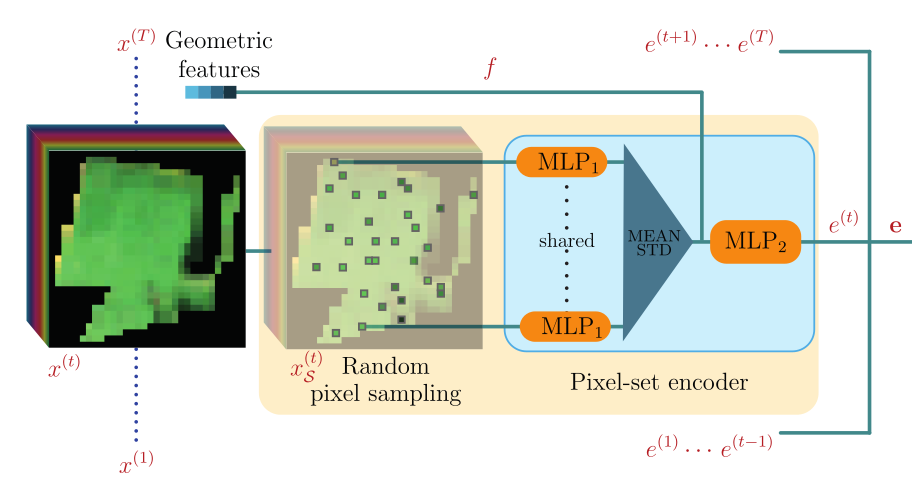
\includegraphics[width=0.5\linewidth]{images/how_psetae_works-ga667c28f-d2af-349e-3181-6390db8c0580.png}
    \caption{Spatial pixel set encoder\cite{garnot_satellite_2020}}
    \label{fig:PSE}
\end{figure}

Jia et al. \cite{jia_graph--graph_2024} proposed an innovative approach using ensemble learning that combines internal and external graph convolutions. This is illustrated in Figure \ref{fig:GIGCN} This method, known as the Graph in Graph Convolutional Network (GiGCN), is designed to extract hierarchical features from both internal and external graphs through two specific processes: Internal Graph Convolution (IGC) and External Graph Convolution (EGC).

\begin{figure}[h]
    \centering
    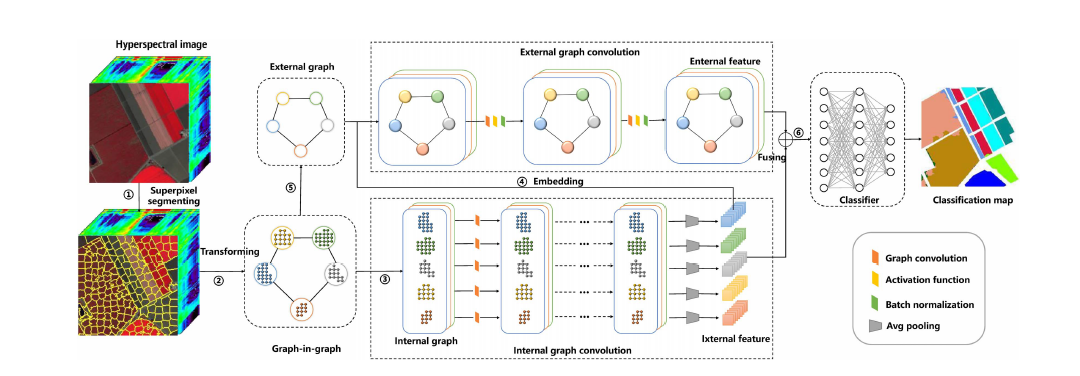
\includegraphics[width=1\linewidth]{images/GIGCN.PNG}
    \caption{A schematic framework of the Graph in Grap Convolution Network\cite{jia_graph--graph_2024}.}
    \label{fig:GIGCN}
\end{figure}
The IGC focuses on extracting local spectral and spatial texture features within each superpixel. By adapting to the natural boundaries of superpixels, IGC eliminates the need for regular shapes and sizes.Conversely, the EGC extracts global features by analyzing the relationships between adjacent superpixels. This approach captures the overall structure and context of the superpixels, adding spatial constraints that help to overcome the issue of spectral variability.

Together, these features interact iteratively within the network, generating a comprehensive and integrated feature vector that combines both local and global characteristics. This results in a more robust and detailed feature representation.

\section{Graph Neural Networks}
The example of GIGCN illustrates how graph-based neural networks utilize global context to improve the accuracy of semantic inference. Real-world objects rarely conform to regular shapes and often display complex spatial relationships. Similarly, datasets in domains like social networks and transportation applications present intricate connectivity patterns that defy representation and analysis using Euclidean geometry. Consequently, methods capable of handling non-Euclidean data become essential. Graph neural networks serve as such methods that specialize to graph data.

\subsection{Graph data}
Graph-based representations capture and convey detailed information about the spatial relationships and contextual dependencies present in the data. Traditional methods like pixel-based or grid-based representations may struggle to capture these complexities. In the context of ground objects, which can vary significantly in shape, size, and spatial arrangement, representing them as nodes and edges in a graph allows for a more nuanced and comprehensive understanding of their characteristics.

A graph is mathematically represented as $G=(V, E)$ where $V = \{u_i\}_{i=1}^N$ is a set with $N$ nodes and $E = \{(u, v)\}$ is an edge set in which the node $u \in V$ connects to the node $v \in V$.
The object's attributes are encoded on the nodes as node features and the relationships between different parts of an object on edges. This effectively captures the structural and contextual information\cite{jia_graph--graph_2024}.

What differentiates graph data from the traditional grid structure, like in images where each pixel has a consistent set of neighboring pixels, in graph data, the structure is not consistent. The number of neighbors for each node can vary, and the connections between nodes are not constrained to a fixed pattern\cite{daigavane_understanding_2021}.

The models that specialize on graph data have to have two essential characteristics, they  must preserve the relationships between graph entities as defined by the adjacency matrix. The connections between nodes should be preserved throughout the model's computations. Second, they should be permutation invariant. This means that the model's predictions should not be affected by the ordering of nodes or edges in the graph. The output should remain the same even if the ordering of nodes are rearranged\cite{sanchez-lengeling_gentle_2021}. 



\subsection{How GNNs work}
The structure of graphs allows us to solve a variety of tasks, including node classification, graph classification, node clustering, link prediction, and influence maximization (where we identify influential nodes).

Generally, Graph Neural Networks (GNNs) use a message passing mechanism so that each node is aware of its context in the graph as well as having information about its neighbors. Consider a graph \( G \) with \( N \) nodes and \( E \) edges, where each node \( v_i \) has a feature vector or embedding \( \mathbf{h}_i \).

For example, focusing on node \( A \) in Figure \ref{fig:Message passing} 
\begin{figure}[h]
    \centering
    \includegraphics[width=0.45\textwidth]{sample_image.png}
    \caption{Illustration of a graph}
    \label{fig:Message passing}
\end{figure}

with features \( \mathbf{h}_A = [x_1, x_2, x_3] \), its direct neighbors are nodes \( B \) and \( F \), both also having feature vectors \( \mathbf{h}_B = [x_1, x_2, x_3] \) and \( \mathbf{h}_F = [x_1, x_2, x_3] \). The first step in message passing for node \( A \) involves gathering the embeddings of all its neighboring nodes using a function \( g \). This can be represented as:

\[
\mathbf{m}_A = g(\mathbf{h}_B, \mathbf{h}_F)
\]

These gathered embeddings \( \mathbf{m}_A \) are then aggregated, typically via sum or mean, preserving the same feature vector size. This aggregation step is known as pooling. For instance, if we use sum aggregation:

\[
\mathbf{m}_A = \mathbf{h}_B + \mathbf{h}_F
\]

or if we use mean aggregation:

\[
\mathbf{m}_A = \frac{\mathbf{h}_B + \mathbf{h}_F}{2}
\]

The pooled embedding are then passed through an update function, usually a neural network. This can be represented as:

\[
\mathbf{h}'_A = \text{MLP}(\mathbf{h}_A, \mathbf{m}_A)
\]

where \( \text{MLP} \) denotes a multi-layer perceptron as the update function.

This process is repeated for all nodes in the graph to generate updated embedding. The message passing steps are repeated based on the number of layers in the network, ultimately allowing each node to learn about the features of all other nodes in the graph. However, this can lead to a problem known as over-smoothing, where nodes become indistinguishable from each other if the network has too many layers.

The updated final embedding are then passed through a classifier to make a prediction. In some instances, pooling may be required before classification as well. For example, given node features with a task of graph classification, it will be necessary to pool the node embedding to produce a global vector that represents the entire graph. This can be achieved by summing or averaging the node embedding:

\[
\mathbf{h}_{\text{global}} = \text{Pooling}(\{\mathbf{h}'_i \mid i = 1, \ldots, N\})
\]

where the pooling function can be a sum or mean operation, aggregating the node embeddings into a single global vector. This global vector is then used for classification of the entire graph:

\[
\hat{y} = \text{Classifier}(\mathbf{h}_{\text{global}})
\]

This allows the model to make predictions based on the overall structure and features of the graph. This simple GNN is illustrtaed in Figure \ref{fig:Simple GNN}
\begin{figure}
    \centering
    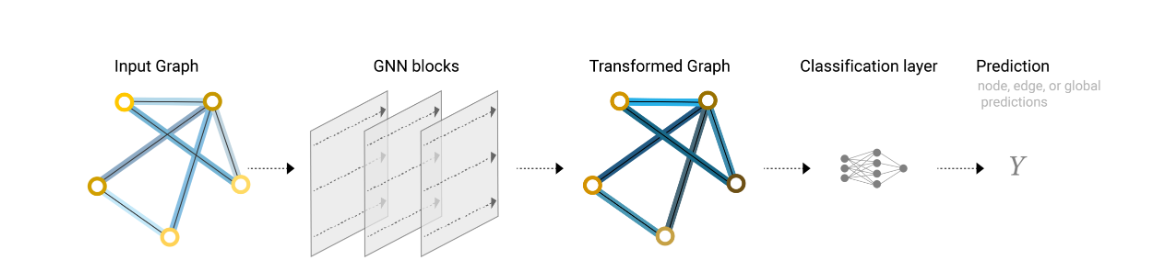
\includegraphics[width=1\linewidth]{images/general gnn.PNG}
    \caption{ A simple GNN frameworkv\cite{sanchez-lengeling_gentle_2021}}
    \label{fig:Simple GNN}
\end{figure}



\subsubsection{Graph Convolution Network}
The message passing is the building block for various GNN architectures, each defining AGGREGATE and UPDATE functions. In the GCN architecture, the update function within the message passing mechanism is the convolutional operator\cite{zhou_graph_2020}. Traditionally, CNNs apply convolutional filters or kernels across the data. These filters slide over the input data and compute dot products between the filter and local regions of the input. The filter's size and the stride determine the receptive field, meaning each output value is influenced by a specific local region of the input. For Graph Convolutional Network (GCN) , the convolution operation is generalized to graphs. Each node aggregates features from its neighbors and itself to compute its new feature representation.
The updated feature of node \(i\) in a GCN is given by:

\[
\mathbf{h}_i' = \sigma \left( \sum_{j \in \mathcal{N}(i)} \frac{1}{c_{ij}} \mathbf{W} \mathbf{h}_j \right)
\]

where:
\begin{itemize}
    \item \(\mathbf{h}_i'\) is the updated feature of node \(i\),
    \item \(\mathcal{N}(i)\) is the set of neighbors of node \(i\),
    \item \(c_{ij}\) is a normalization constant,
    \item \(\mathbf{W}\) is a weight matrix, and
    \item \(\sigma\) is a non-linear activation function such as ReLU\cite{kipf_semi-supervised_2017}.
\end{itemize}
Neighborhood aggregation enables a Graph Convolutional Network (GCN) to capture patterns in the local neighborhood of nodes. If a GCN learns to recognize specific subgraph structures, it can generalize this knowledge to identify similar patterns elsewhere in the graph. This is analogous to how Convolutional Neural Networks (CNNs) recognize image features like edges or textures.

Enhancing GNNs performance can be achieved both by architectural modifications, or by enriching the features of the graphs themselves. One significant modification to the GCN architecture is the application of an attention mechanism to each node’s neighborhood. Unlike GCNs, which apply the same weight matrix to all node features and their neighbors, the attention mechanism assigns different weights to each neighbor. This approach allows the model to assign different importance to nodes within the same neighborhood, thereby enhancing the model's capacity to focus on the most relevant nodes while aggregating features. This modification is known as the Graph Attention Network (GAT) \cite{velickovic_graph_2018}.

Graph representations on the other hand can be improved by making graphs more feature-rich leading to better model performance, even with existing models. For instance, incorporating spatial information in the nodes can provide more context and the graph becomes a more comprehensive representation of the underlying data.


\subsubsection{Spatial information and Graph Convolution}
Danel et al. \cite{danel_spatial_2020} proposed Spatial Graph Convolutional Network (SGCN), a generalization of GCN. In this network, node positions, represented as two-dimensional pixel coordinates, were added as an additional node feature, thus incorporating spatial information into the aggregation process. This inclusion of geometric information enhances the model's ability to understand the spatial or geometric relationships between nodes in the graph. This takes the form 

\[
\mathbf{h}_i' = \sigma \left( \sum_{j \in \mathcal{N}(i)} \frac{1}{c_{ij}} \mathbf{W} \mathbf{h}_j + \mathbf{W}_p (\mathbf{p}_j - \mathbf{p}_i) \right)
\]

where:
\begin{itemize}
    \item \(\mathbf{h}_i'\) is the updated feature of node \(i\),
    \item \(\mathcal{N}(i)\) is the set of neighbors of node \(i\),
    \item \(c_{ij}\) is a normalization constant,
    \item \(\mathbf{W}\) is a weight matrix for node features,
    \item \(\mathbf{W}_p\) is a weight matrix for spatial features,
    \item \(\mathbf{p}_i\) and \(\mathbf{p}_j\) are the coordinates of nodes \(i\) and \(j\) respectively,
    \item \(\sigma\) is a non-linear activation function such as ReLU \cite{danel_spatial_2020}.
\end{itemize}


TODO
How to keep spatial information in the nodes:
- consider node (relative) position as a node feature
- consider node position as a way to add geometry into the graph convolution (\url{https://arxiv.org/pdf/1909.05310}, \url{https://www.researchgate.net/profile/Agnieszka-Slowik-5/publication/335788572_Geometric_Graph_Convolutional_Neural_Networks/links/5d81a00b458515fca1711ef9/Geometric-Graph-Convolutional-Neural-Networks.pdf})


%\bibliography{Thesisref}